\chapter{Background} \label{ch:background}
As described in the research proposal for this project, several GEC shared tasks at the beginning of this decade led to significant advances in research: the Helping Our Own (HOO) shared tasks in 2011 and 2012 \citep{Dale2011HelpingTask, Dale2012HOOTask}, and the shared tasks at the 17th and 18th conferences on Computational Natural Language Learning (CoNLL) in 2013 and 2014 \citep{Ng2013TheCorrection, Ng2014TheCorrection}. In this timeframe, a new task-specific scoring framework was developed \citep{Dahlmeier2012BetterCorrection} and the spotlight shifted from highly linguistically motivated and error-specific classifiers and rule-based methods to more generalized machine translation techniques. Error-specific approaches, while they require more linguistic expertise and model complexity to achieve full coverage of grammatical error types, have the advantage of performing particularly well on the specific error types they target. On the other hand, statistical machine translation (SMT) methods have achieved state-of-the-art results on GEC, capturing complex interactions between different error types without requiring the individual construction of as many component models. Some have even attempted to combine the advantages of each technique with hybrid systems \citep{Susanto2014SystemCorrection,Rozovskaya2016GrammaticalClassifiers}.

Meanwhile, machine translation (MT) has experienced its own revolution, from the advent of neural machine translation (NMT) methods around 2013 and 2014 \citep{Kalchbrenner2013RecurrentModels,Cho2014LearningTranslation,Cho2014OnApproaches,Sutskever2014SequenceNetworks} to their adoption by Google and Microsoft last year \citep{Wu2016GooglesTranslation}. While many GEC researchers have continued to improve the performance of phrase-based SMT \citep{Junczys-Dowmunt2016Phrase-basedCorrection,Chollampatt2016NeuralCorrection} and hybrid classifier-SMT systems \citep{Susanto2014SystemCorrection,Rozovskaya2016GrammaticalClassifiers}, those pioneering the application of NMT methods to GEC \citep{Xie2016NeuralAttention,Yuan2016GrammaticalTranslation} have not been able to meet the state-of-the-art performance according to the accepted scoring method using the MaxMatch scoring framework, presented in the next section.

\section{MaxMatch Scorer}
Establishing a standard evaluation metric is key to building on prior work and making progress on any research topic. The way that GEC systems have been evaluated in most recent work can be broken down to two components: first, a method to align a pair of sentences and extract the edits necessary to transform the given input to the given output; second, a scoring function based on Levenshtein edit operations (insertion, deletion, and substitution) to assess the accuracy of the transformation, typically an $F$ score between the extracted edits and a set of gold standard edits.

\subsection{Alignment}
% TODO: alignment problem vs scoring function, why is alignment an important task?
There is often more than one way to align two sentences and identify a set of edits that represent their differences. There can be more than one possible set of token-level edits leading to the same resulting sentence, but there can also be phrase-level edits on top of these, resulting in some ambiguity around which system edits to feed into the scoring function.

\citet{Dahlmeier2012BetterCorrection} illustrate the problem with an example from the 2011 HOO shared task:

\begin{table}[h]
\centering
\begin{tabular}{ r l }
\tabularnewline \hline \hline
Source & Our baseline system feeds word into PB-SMT pipeline. \\
Hypothesis & Our baseline system feeds \textbf{a} word into PB-SMT pipeline. \\
\hline
\end{tabular}
\caption{Example of ambiguous edit extraction from HOO 2011: is the edit an insertion of the token \texttt{a}, the substitution of the token \texttt{word} with the phrase \texttt{a word}, or something else?}
\label{tab:maxmatch-hoo-2011-example}
\end{table}

The official evaluation script of the shared task extracts the edit $\epsilon \rightarrow \texttt{a}$, while the gold standard annotation is $\texttt{word} \rightarrow \texttt{\{a word, words\}}$. Even though both edits could produce the same output string, there is no overlap between the extracted system edit and the gold standard edit choices, so the hypothesis is considered incorrect.

% However, identifying system edits from a pair of input and output texts proved ambiguous in cases where a proposed edit resulted in the correct output string but did not correspond to an edit in the gold standard set. For example, given an input sentence, ``I'm craving burger,'' and system output, ``I'm craving a burger,'' if the gold standard edits were $\texttt{burger} \rightarrow \texttt{\{a burger, burgers\}}$, the HOO scorer would deterministically extract as a system edit $\epsilon \rightarrow \texttt{a}$ (insertion of the word `a') regardless of the gold standard edits. Even though the results of the proposed system edit and of one of the gold standard choices are the same, the HOO evaluation framework would underestimate the system's performance.

To solve this problem, \citet{Dahlmeier2012BetterCorrection} designed the MaxMatch ($M^2$) scoring system to choose from ambiguous system edit possibilities in order to maximize the overlap between system and gold standard edits. The $M^2$ scorer first constructs an edit lattice by filling in a matrix with the Levenshtein distances between substrings of the tokenised input and output and computing all shortest paths through the matrix that transform the input sentence into the system output. Table \ref{tab:maxmatch-levenshtein-matrix} depicts the Levenshtein matrix between source \texttt{i studying informatic .} and hypothesis \texttt{i am studying informatics .}

\begin{table}[h]
\centering
\begin{tabular}{|r|c|c|c|c|c|c|}
\hline
 &  & i & am & studying & informatics & . \\ \hline
 & 0 & 1 & 2 & 3 & 4 & 5 \\ \hline
i & 1 & 0 & 1 & 2 & 3 & 4 \\ \hline
studying & 2 & 1 & 1 & 1 & 2 & 3 \\ \hline
informatic & 3 & 2 & 2 & 2 & 2 & 3 \\ \hline
. & 4 & 3 & 3 & 3 & 3 & 2 \\ \hline
\end{tabular}
\caption{Levenshtein matrix between \texttt{i studying informatic .} and \texttt{i am studying informatics .}}
\label{tab:maxmatch-levenshtein-matrix}
\end{table}

The shortest paths are represented as a graph with each node corresponding to a cell from the Levenshtein matrix and each edge corresponding to an edit operation: insertion, deletion, substitution, or no change. Since GEC data annotations sometimes include phrase-level like $\texttt{studying} \rightarrow \texttt{am studying}$ for the example above, the alignment framework should also allow some phrase-level edits in which some words remain unchanged. However, it should do so within reason, without allowing edits spanning long sequences in which many words remain unchanged, so the number of permitted unchanged words in an edit is limited by a parameter (a reasonable default is 2). These additional edits are added to the edit lattice as new edges that combine adjacent existing edges, as illustrated in \ref{fig:maxmatch-edit-lattice}.

\tikzstyle{unit}=[circle, minimum size=1.2cm, draw=black, inner sep=0pt]

\begin{figure}[h]
\centering
  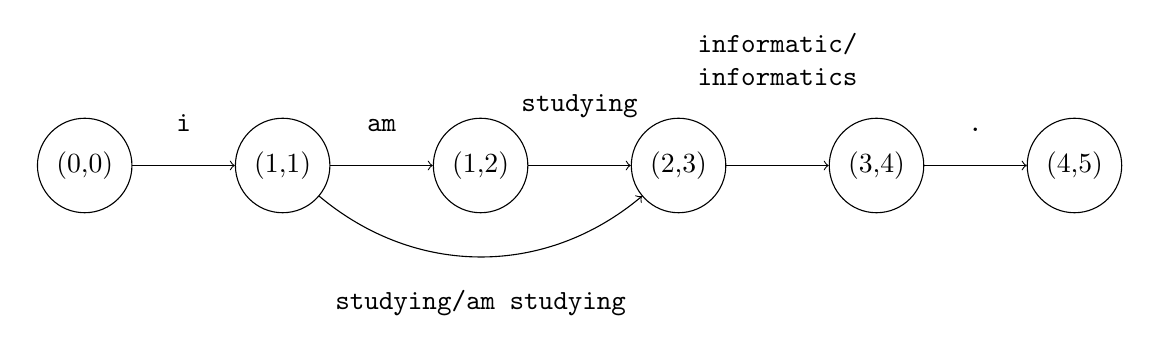
\begin{tikzpicture}[el/.style = {inner sep=2pt, align=left, sloped}, every label/.append style = {font=\footnotesize}]
    \matrix[row sep=1cm,column sep=1.3cm] {
      \node (0) [unit] {(0,0)}; &
      \node (1) [unit] {(1,1)}; &
      \node (2) [unit] {(1,2)}; &
      \node (3) [unit] {(2,3)}; &
      \node (4) [unit] {(3,4)}; &
      \node (5) [unit] {(4,5)};\\
    };
    
    \path[->]
    (0) edge node[el,above,yshift=10] {\texttt{i}} (1)
    (1) edge node[el,above,yshift=10] {\texttt{am}} (2)
    (1) edge [bend right=40] node[el,below,yshift=-10] {\texttt{studying/am studying}} (3)
    (2) edge node[el,above,yshift=15] {\texttt{studying}} (3)
    (3) edge node[el,below,yshift=50] {\texttt{informatic/}\\\texttt{informatics}} (4)
    (4) edge node[el,above,yshift=10] {\texttt{.}} (5);
  \end{tikzpicture}
\caption{Edit lattice from source \texttt{i studying informatic .} to hypothesis \texttt{i am studying informatics .}}
\label{fig:maxmatch-edit-lattice}
\end{figure}

\subsection{Edit Extraction}
Based on this edit lattice, the $M^2$ scorer chooses the complete set of edits from input to output which maximally match the set of gold standard edits. Matches are defined as any edit with the same start and end position in the input sentence and with proposed correction included in the gold standard correction.

\subsection{Scoring Function}
Initially, GEC researchers continued using $F_1$ as the scoring function with the results of $M^2$ alignment and edit extraction, but beginning with CoNLL-2014, it became standard to use the $F_{0.5}$ score (for reasons mentioned in chapter \ref{ch:intro}), and $M^2$ score became synonymous with $M^2$ edit extraction followed by $F_{0.5}$ score.

\section{GEC Approaches}
We can look to the CoNLL shared tasks of 2013 and 2014 to sample the range of possible approaches to GEC. These shared tasks not only popularised the $M^2$ scoring framework but also introduced datasets that would continue to be used commonly in GEC research to this day.

\subsection{Classifiers}
One of the most popular approaches among submissions to CoNLL-2013 was error-specific machine learning classifiers, one for each of the five grammatical error types included in the task. Five of the submissions were systems based on maximum entropy; others used Naive Bayes, SVMs, perceptrons, and other classifiers. The system with the best $F_1$ score on the test set (42.14\%) consisted of a multi-class averaged perceptron for article or determiner errors, and Naive Bayes for the remaining error types (preposition, noun number, verb form, and subject-verb agreement errors).

Machine learning classifiers remained a common approach in the CoNLL-2014 submission, though almost always in combination with other approaches so as to increase coverage of the 28 error types included in the task. The second best $F_{0.5}$ score on the test set (26.79\%), in spite of handling only nine of the 28 error types, was achieved by a system using ``different combinations of averaged perceptron, Naive Bayes, and pattern-based learning trained on different data sets for different error types'' \citep{Ng2014TheCorrection}.

\subsection{Rule-Based}
Four CoNLL-2013 submissions were rule-based classifiers and two hybrid systems included rule-based components in a pipeline with other methods. CoNLL-2014 similarly included rule-based approaches, but usually mixed with other approaches. The highest $F_{0.5}$ score achieved in CoNLL-2014 (37.33\%) was by a system using rule-based classifiers as a first pass, followed by four steps of ranking hypotheses based on language model probabilities, statistical machine translation, LM ranking again, and type filtering. Hand-crafted rules require extensive linguistic domain expertise Needless to say, purely rule-based techniques no longer appear among the best performing GEC systems.

\subsection{Language Models}
As mentioned for the best performing submission to CoNLL-2014, using language model probabilities to rank hypotheses is another approach, often implemented as a component in a more complex system. It conveniently does not require an annotated grammatical error correction corpus to train an n-gram language model, simply a corpus of grammatically correct text. The result is a way of not only possibly generating new grammatical hypotheses but also comparing their correctness to the source sentence to ensure an improvement.

% CoNLL-2013 also introduced the datasets that are commonly used for GEC until today (described more fully in section \ref{sec:datasets}) and 
% The CoNLL shared tasks of 2013 and 2014 popularised the use of the $M^2$ scoring framework and witnessed a range of methods for GEC, much of which came to dominate how GEC research is done today.
% TODO: why do we care? they introduce the datasets (ref section) and there are other approaches besides machine translation (e.g. CoNLL briefly)

% The CoNLL-2013 shared task covered only five grammatical error types: article or determiner errors, preposition errors, noun number errors, verb form errors, and subject-verb agreement errors. The majority of systems built by the sixteen teams who submitted descriptive papers were error-specific classifiers. Some classifiers were trained on examples that encoded the context in which each error type occurred, some used hand-crafted deterministic rules, and some were built with a combination of the two approaches. A handful of systems were built using machine translation approaches, both phrase-based and syntax-based statistical machine translation, and two systems used language modeling to choose a corrected sentence that is more likely than the uncorrected sentence. These different approaches are also used in combination, in some cases set up as a pipeline to handle different error types with different GEC systems.

% The CoNLL-2014 shared task expanded coverage to include all 28 error types annotated in its training dataset (NUCLE, the same training dataset used for CoNLL-2013). Additional error types included verb tense errors, pronoun reference errors, wrong idioms, etc. Including such varied error types that potentially interact in complicated ways made it much harder to approach the task one error type at a time. As a result, there was a greater prevalence of error-agnostic approaches such as language modeling and machine translation (phrase-based only this time, not syntax-based) among the systems implemented by the twelve teams who submitted system description papers. The submission with the best $F_{0.5}$ score used a pipeline of deterministic rules, language model ranking, and SMT.

\section{The Machine Translation Approach}
When CoNLL-2014 increased coverage from five to 28 error types, systems based on error-specific approaches like machine learning and rule-based classifiers became somewhat less practical to build and a larger portion of submissions turned to machine translation techniques, which frame GEC as the translation of ungrammatical text into grammatical text.
% With the 2013 and 2014 CoNLL shared tasks, work in grammatical error correction started shifting more toward machine translation techniques. GEC can be framed as the translation of ungrammatical text into grammatical text.

In this section, we use the usual MT terminology of translating a foreign/source sentence $f$ into an English/target sentence $e$, except in GEC both source and target are in English and the source sentence $f$ may have grammatical errors while the target sentence $e$ has none.

\subsection{Statistical Machine Translation}
The problem of statistical machine translation can be posed using the noisy channel framework and Bayes' Rule as finding the most likely translation $\hat{e}$ for a sentence $f$ in a foreign language:
\begin{equation} \label{eq:bayes}
	\hat{e}=\underset{e}{\arg\!\max}\ p(e|f)=\underset{e}{\arg\!\max}\ p(e)p(f|e)
\end{equation}
This formulation breaks the system down to two components: a language model $p(e)$ and a translation model (or conditional language model) $p(f|e)$. As the probability of a particular sequence of words occurring in a particular order, the language model represents how correct the target sentence is. \citet{Zens2002Phrase-basedTranslation} further breaks down the translation model into a lexicon and an alignment model.

% TODO: delete? who cares about word-based SMT?
In word-based SMT, the translation probability $p(f|e)$ can be represented with an optional sentence length probability, in addition to lexicon probabilities and alignment probabilities:
\begin{equation} \label{eq:word-based}
	p(f|e)=p(J|e)\sum_{a}\prod_{j=1}^{J}[p(f_j|e_{a_j})p(a_j|a_{j-1},I,J)]
\end{equation}
where $J$ and $I$ are the lengths of the source and target sentences $f$ and $e$, respectively, and $a_j$ is the index of the target word aligned to source word $f_j$. The lexicon probability $p(f_j|e_{a_j})$ is the probability that source word $f_j$ translates to target word $e_{a_j}$. The alignment probability $p(a_j|a_{j-1},I,J)$ is the probability that the position of source word $f_j$ maps to the position of target word $e_i$, given the alignments of previous words in the source sentence and the lengths of the source and target sentences.

In phrase-based SMT, the segmentation of the sentence pair into $K$ phrases is an additional hidden variable $B$. Assuming all segmentations have the same probability and allowing only monotone translations:
\begin{equation} \label{eq:phrase-segmentation}
	p(f|e)=\prod_{k=1}^{K}p(f_k|e_k)
\end{equation}
where each phrase translation probability $p(f_k|e_k)$ is estimated by its relative frequency:
\begin{equation} \label{eq:phrase-translation-prob}
	p(f_k|e_k)=\frac{N(f_k,e_k)}{N(e_k)}
\end{equation}
These are counts in the training corpus: $N(e_k)$ is the number of times the phrase $e_k$ occurred, $N(f_k,e_k)$ the number of times $f_k$ appeared as a translation of $e_k$. Once counted (trained), these estimated probabilities are looked up in a phrase translation table for decoding.

Combining Equations \ref{eq:bayes}, \ref{eq:phrase-segmentation}, and \ref{eq:phrase-translation-prob}, as well as a translation model scaling factor $\lambda$ (to indicate relative importance of language model and translation model contributions), the task of monotone translation becomes something more like this:
\begin{equation} \label{eq:stat-mt-summary}
	\hat{e}=\underset{e,B}{\arg\!\max}{\prod_{i=1}^{I}p(e_i|e_1,e_2,...,e_{i-1}) \prod_{k=1}^{K}p(f_k|e_k)^\lambda}
\end{equation}

For non-monotone translations, the task also includes a distance-based phrase reordering (or distortion) probability $d$ \citep{koehn2009statistical}:
\begin{equation} \label{eq:stat-mt-distortion-summary}
	\hat{e}=\underset{e}{\arg\!\max}{\prod_{i=1}^{I}p(e_i|e_{<i})^{\lambda_{LM}} \prod_{k=1}^{K}p(f_k|e_k)^{\lambda_{\phi}}}d(start_i-end_{i-1}-1)^{\lambda_{d}}
\end{equation}
Each feature has a relative weight $\lambda$ that must be learned through training.

% TODO: more features? see statmt/Moses wiki on Scoring Phrases: http://www.statmt.org/moses/?n=FactoredTraining.ScorePhrases

% this is where it starts going wrong
% In \cite{Koehn2003StatisticalTranslation}, there is a third component $\omega^{\texttt{length}(e)}$, where generally $\omega>1$ to bias the system to produce longer output sentences as a way of ``calibrating'' the source and target sentence lengths (much like the standard metric for machine translation, BLEU, penalizes short translations). In phrase-based translation, the translation model (TM) operates at the phrase level such that the probability $p(f|e)$ for the whole sentence can be broken down further:
% \begin{equation}
% 	p(f|e)=\prod_{i=1}^{I}p(f_i|e_i)d(a_i-b_{i-1})
% \end{equation}
% where $I$ is the number of phrases in the segmented foreign sentence $f$, so $f_i$ and $e_i$ are respectively the foreign and English phrases corresponding to the $i$th phrase of the foreign sentence, and $d$ is a distortion model that captures any phrase reordering that should occur as a result of translation.

% decoder, beam search
% training

% \subsubsection{Features} %TODO

\subsubsection{Hybrid Classifier-SMT Systems for GEC}
% Susanto et al. (2014)
\citet{Susanto2014SystemCorrection} surpassed the performance of the best system from CoNLL-2014 using a hybrid system with both error-specific classifiers and SMT. Their best reported $F_{0.5}$ score of 39.39\% on the test data from CoNLL-2014 resulted from a combination of four independent GEC systems: two that were pipelines of classifier-based correction steps of six common error types (spelling errors, noun number errors, preposition errors, punctuation errors, article errors, and verb form or subject-verb agreement errors) and two that were SMT models. The pipeline systems differed in the order of the correction steps (swapped noun number and article errors), and the SMT systems differed in phrase table construction (two phrase tables built from two separate corpora versus one phrase table built from the concatenation of the two corpora). Three of the six correction steps used classifiers learned from context features for noun number, prepositions, and articles; two were rule-based classifiers to fix punctuation errors and subject-verb agreement errors; and the first correction step was the output of an open source spell-checker (Jazzy), whose output was filtered using language model probabilities. Neither individual systems nor combinations of one pipeline and one SMT system each could match the performance of the combination of all four systems. The recall of the four-part system was 19.14\%, but the two pipeline systems achieved 23.99\% and 22.77\% individually

% Rozovskaya & Roth (2016)
More recently, \citet{Rozovskaya2016GrammaticalClassifiers} far surpassed even this performance with a classifier-SMT model combination that scored 47.40\% on the CoNLL-2014 test set (recall of 25.64\%). The classifier used in the final system combination was initially trained on native data, i.e. a corpus of text assumed to be grammatically correct, then ``tailored'' by artificially introducing grammatical error patterns from a learner corpus, and finally further enhanced by introducing mechanical errors in punctuation, spelling, and capitalization. By running the classifier's output through an SMT system trained on the Lang-8 parallel corpus, they pushed the state-of-the-art to 8 percentage points more than \citet{Susanto2014SystemCorrection}.

\subsubsection{SMT Systems for GEC}
% Mizumoto & Matsumoto (2014)

% Chollampatt et al. (2016)

% Junczys-Dowmunt & Grundkiewicz (2016)
The state of the art in GEC at the time of this writing was set by \citet{Junczys-Dowmunt2016Phrase-basedCorrection} with an SMT system tuned to the GEC-specific $M^2$ metric, i.e. the same $F_{0.5}$ score used to evaluate GEC systems since CoNLL-2014, rather than to the MT-oriented BLEU score as in \citet{Susanto2014SystemCorrection} and \citet{Rozovskaya2016GrammaticalClassifiers}.

Tuning to $M^2$ with a standard phrase-based SMT system resulted in an impressive score of 46.37\% on the CoNLL-2014 test data (recall of 25.05\%); when augmented with new GEC-specific features and a large language model trained on the Common Crawl corpus, the system's score increased to 49.49\% (recall of 27.98\%). The GEC features added onto the standard SMT features include stateless (within phrase) features that captured the edits required to transform an input phrase into a candidate output, stateful (phrase context) features that captured the likeliness of a candidate output phrase in the context of the rest of the output sentence, as well as more fine-grained features capturing edit operations between source and candidate target sentences. Such features have not yet been applied in NMT methods for GEC.
% recall: 25.05 baseline, 27.98 with sparse GEC features + LM, but 26.03 baseline without LM, and 26.21 / 28.17 with dense GEC features with / without LM

\subsection{Neural Machine Translation}
Current neural machine translation techniques attempt to model $p(e|f)$ directly without the breakdown of language model and translation model. The general idea behind the encoder-decoder architecture introduced by \citet{Sutskever2014SequenceNetworks}, \citet{Cho2014LearningTranslation}, and \citet{Bahdanau2014NeuralTranslate} is to use an RNN to encode the source sentence into a fixed-length vector, then use another RNN to decode this vector into a target sentence. Since LSTMs and GRUs are better at capturing long-range dependencies in sequences, they are often preferred over vanilla RNNs for tasks such as machine translation.

% TODO: discuss much more detail from Bahdanau et al. (2016) to set up Nematus
% TODO: address NMT comments from IRP (order of n-grams, vocabulary problem, pyramid structure)
\citet{Bahdanau2014NeuralTranslate} proposed an encoder-decoder architecture consisting of a bidirectional LSTM as the encoder and added an attention mechanism to the decoder that behaves somewhat like alignment or distortion in phrase-based SMT to provide a probability distribution over the input positions for any given output position. A context vector calculated at each output position is a weighted average of the encoded representations of each input position, where the weights come from performing a softmax over an alignment model comparing the decoder's hidden state at the previous time step with the encoder's representation at the current time step.
%depend on the alignment probability between the input and output positions.
This attention mechanism removes the requirement that the input sequence be encoded as a fixed-length vector.
% TODO: insert alignment maths

The architecture used in \citet{Xie2016NeuralAttention} included a similar attention mechanism in the decoder and a three-layer bidirectional GRU with a pyramid structure as the encoder to reduce the computational complexity resulting from operating at a character level.

% \subsubsection{Hybrid SMT-NMT?} % TODO
% Junczys-Dowmunt, Dwojak, & Sennrich (2016)

\subsubsection{NMT Systems for GEC}
% Xie et al. (2016)
\citet{Xie2016NeuralAttention} were the first to apply neural machine translation methods to the GEC task, achieving a score of 40.56\% on the CoNLL-2014 test data (recall of 23.77\%). They implemented a character-level encoder-decoder recurrent neural network architecture with attention and a language model to prune translation hypotheses for beam search. Their language model was trained on a subset of the Common Crawl corpus, resulting in 2.2 billion n-grams, only a tiny fraction of the more than 500 billion unique n-grams available in the full corpus \citep{Buck2014NCrawl}. This standard NMT architecture was combined with a mechanism for classifying proposed edits as legitimate or spurious, based on the same understanding mentioned in chapter \ref{ch:intro} that it is preferable that a GEC system fail to suggest an edit than that it make a spurious suggestion. Finally, with data augmentation using two common error types according to error distribution statistics for the CoNLL-2014 training set, their best model outperformed \citet{Susanto2014SystemCorrection} and set the state of the art at the time.

% Yuan & Briscoe (2016)
\citet{Yuan2016GrammaticalTranslation} also tried to apply NMT to GEC, outperforming \citet{Susanto2014SystemCorrection} but falling short of the performance of the best system by \citet{Xie2016NeuralAttention} with a score of 39.90\% on the CoNLL-2014 test data (did not report recall). Their implementation operated on the word level instead of the character level as in \citet{Xie2016NeuralAttention}. However, word-level NMT encounters a problem with handling rare words, due to the necessity of restricting the size of the known vocabulary so as to efficiently perform each word embedding and compute each softmax at the output layer. This problem is exacerbated in GEC since grammatical errors and spelling mistakes necessarily increase the source vocabulary size and are interpreted as extremely rare words any time a particular error is not systematic and widespread. To handle such ``rare words'', they aligned unknown target words to their source words using an unsupervised aligner and applied a word-level translation model learned from IBM Model 4 \citep{Brown1993TheEstimation}. However, it seems this approach to handling the rare word problem may not be as effective as character- or subword-level approach as in \citet{Xie2016NeuralAttention}. % The rest of their attentional encoder-decoder architecture is like Bahdanau et al. (2014) and Xie et al. (2016).